% Part 1

\section{Freeing Absorption Spectrum from Trend and identify Lines}
\label{sec:freeing}
Now we want to free the spectrum from any trend for that the fit a linear function on the spectrum of the reference beam and subtract the fit from the sample beam and reference beam. It is worth mentioning that we have moved the reference beam spectrum down to the niveau of the sample beam spectrum and after that we fitted the linear function. In fig. \ref{image:trends} we can see the absorption spectrum with trends and the linear fit and in fig. \ref{image:trendless} the spectrum without trends. The fit is managed with the function polyfit of the numpy-module in python. We did also cut the data so that we can clearly see the four peaks without any jumps in mode.
\begin{center}
    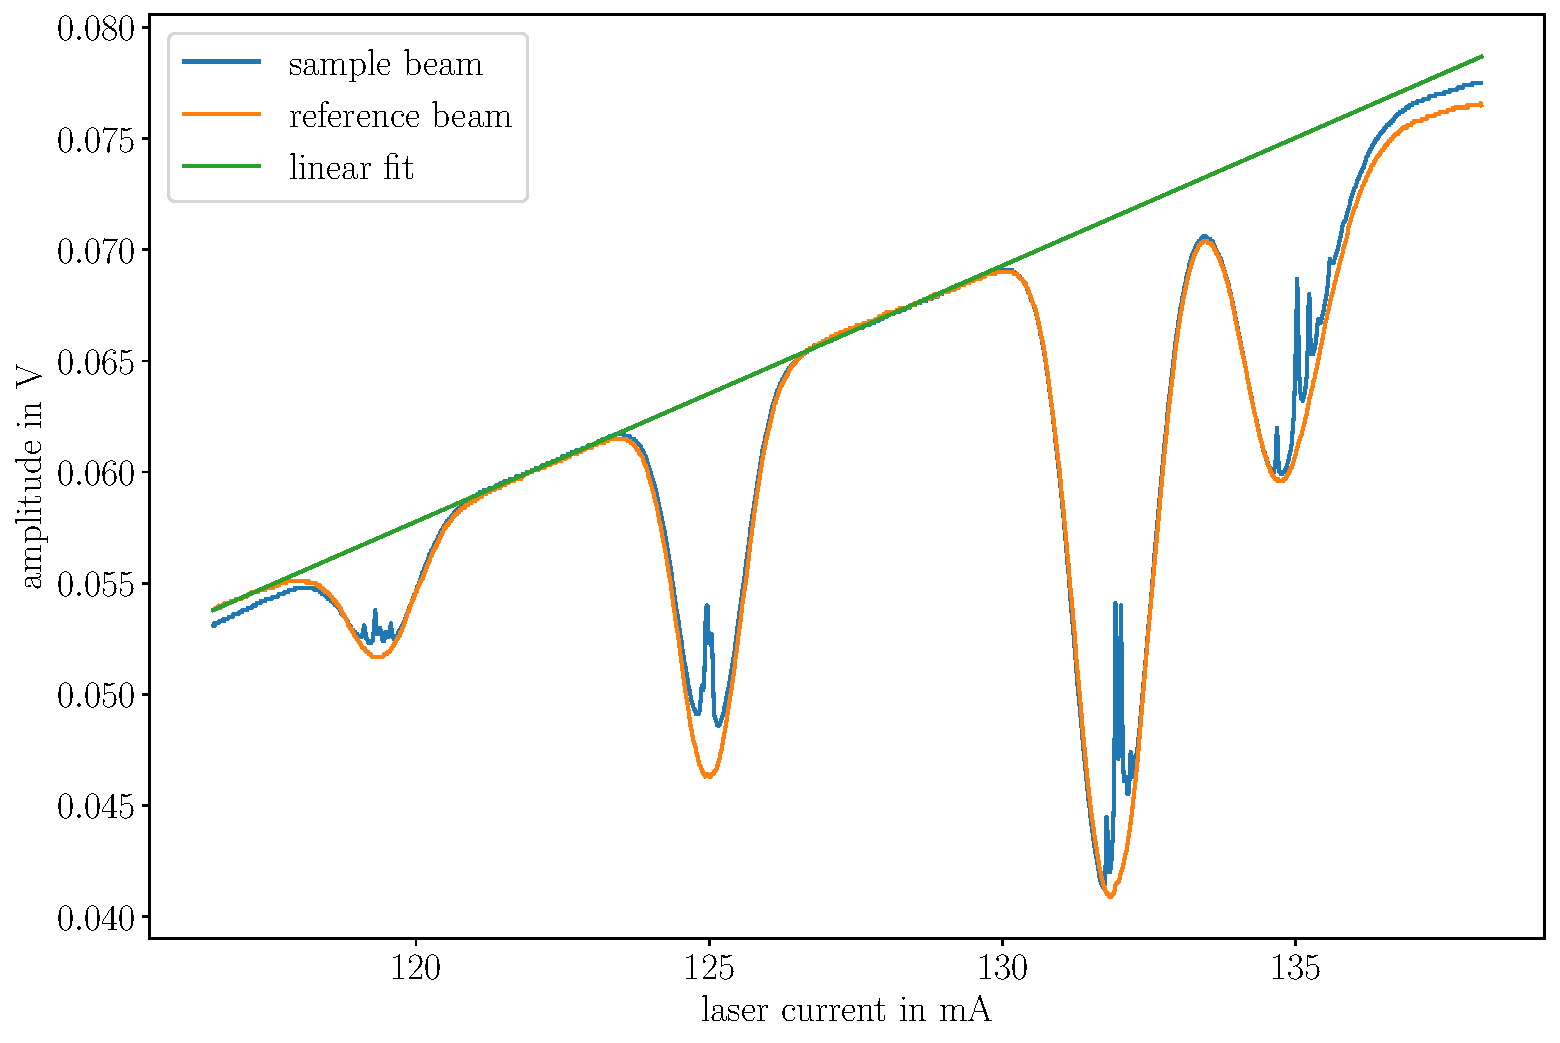
\includegraphics[scale=0.47]{Aufg-1/trend24.pdf}
    \captionof{figure}{Absorption Spectrum with trends}
    \label{image:trends}
\end{center}
\begin{center}
    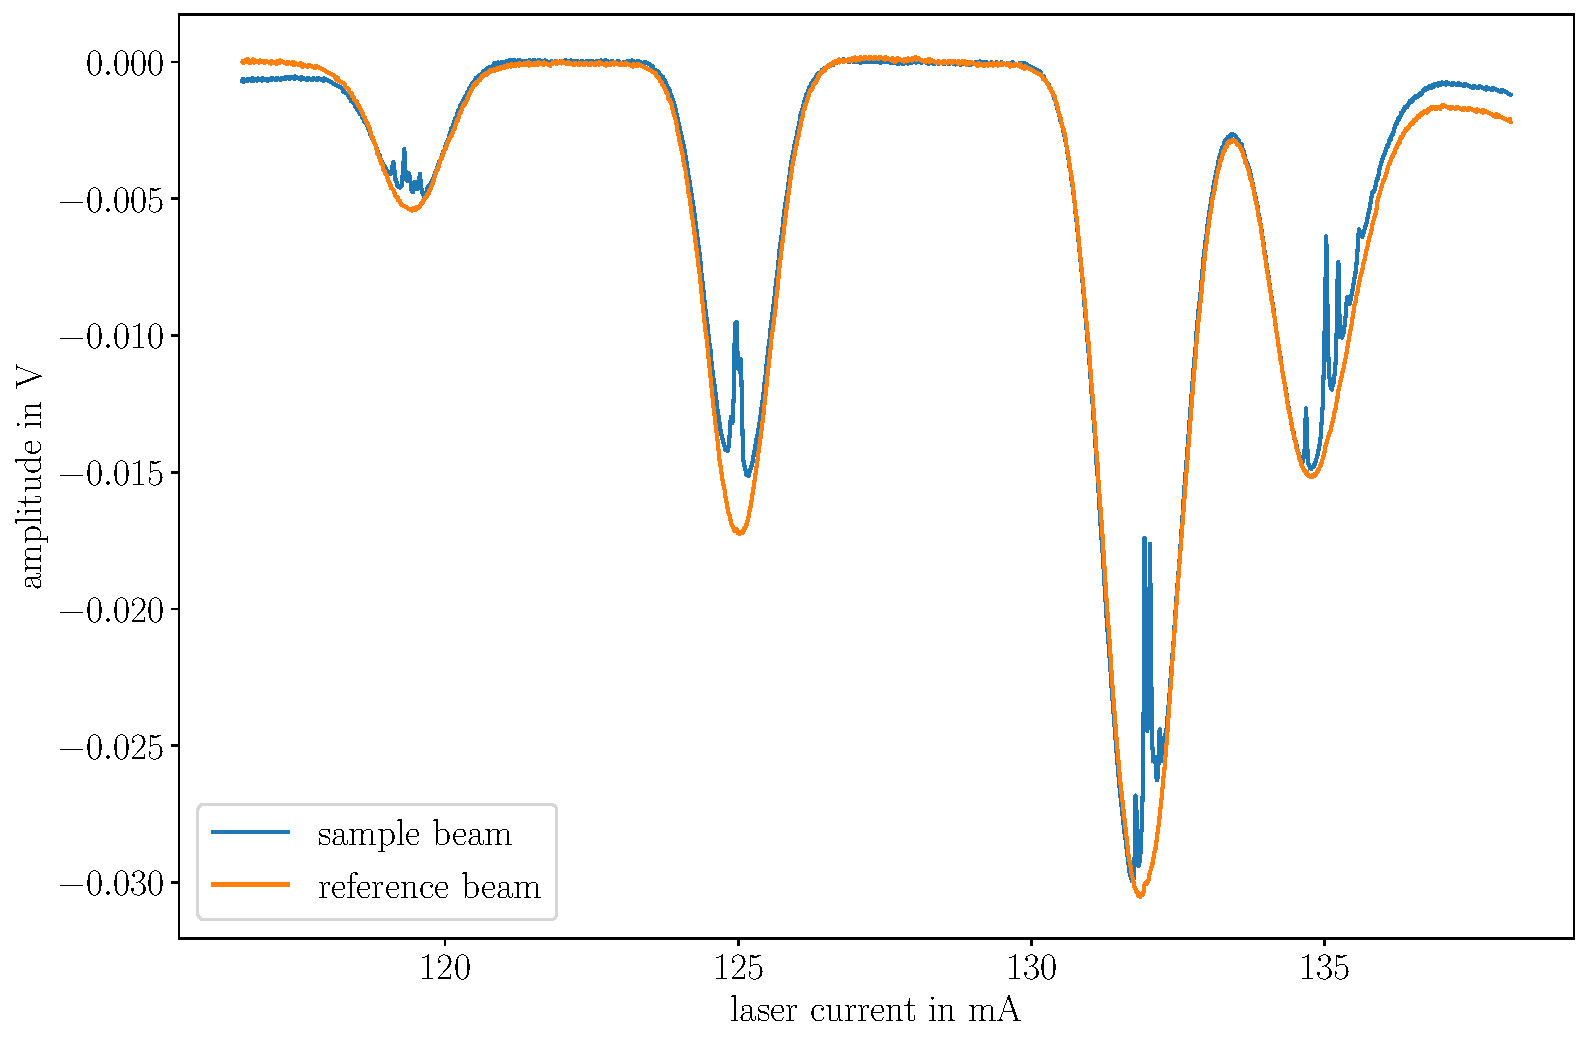
\includegraphics[scale=0.47]{Aufg-1/trendless24.pdf}
    \captionof{figure}{Absorption Spectrum without trends}
    \label{image:trendless}
\end{center}
We applied the same procedure on the data of the fabry-pérot and see clear in fig. \ref{image:allTrendless} that the signal is not very stable, but this is not from interest for the upcoming evaluation because we need only the distance between to peaks.
\begin{center}
    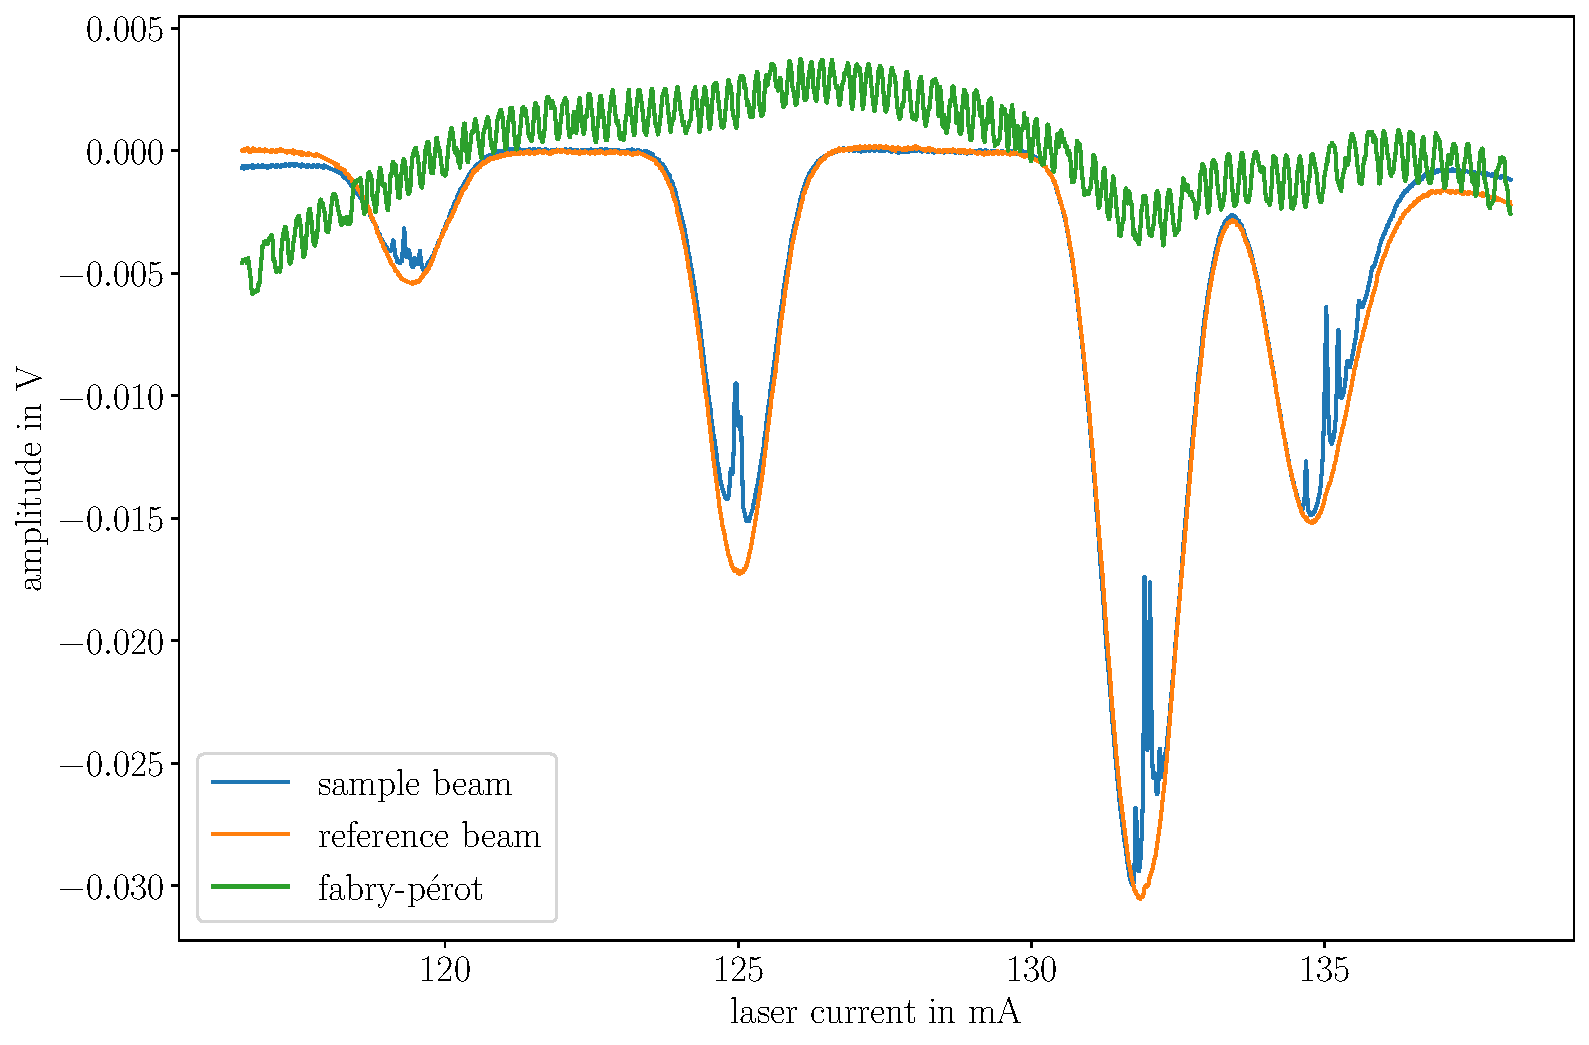
\includegraphics[scale=0.47]{Aufg-1/alltrendless24.pdf}
    \captionof{figure}{Absorption Spectrum without trends all channels}
    \label{image:allTrendless}
\end{center}
\subsection*{Identfication considering intensity and order}
To identify the lines of the spectrum we used the current wavelength curve (look fig. \ref{image:currentTuning}) to convert the laser current to the wavelength. To do this we convert the fig. \ref{image:currentTuning} into a csv-file using python. For that we measured roughly the points of the peaks from 105 mA to 150 mA (because that is the area of interest) and calculated a basic linear function of the form $y=mx +t$ between them (look fig. \ref{image:currentTuningCut}). Then we obtain three separate linear functions that can transform our data in the corresponding wavelength in the specific area of the current wavelength curve.
\begin{center}
    \begin{tabular}{c | c c c c}
        {} & 1 & 2 & 3 & 4 \\
        \hline
        laser current/mA & 107.0 & 128.5 & 129.5 & 149.5\\
        wavelength/nm & 780.23125 & 780.25125 & 780.234 & 780.2535\\
    \end{tabular}
    \captionof{table}{Point used for recreating current wavelength curve}
    \begin{tabular}{c | r r }
        area & m/$\frac{\text{nm}}{\text{mA}}$ & t/nm\\
        \hline
        $1 \rightarrow 2$ & 0.00093  & 780.132 \\
        $2 \rightarrow 3$ & -0.01725 & 782.468 \\
        $3 \rightarrow 4$ & 0.00097  & 780.108 \\
    \end{tabular}
    \captionof{table}{linear functions of the current wavelength curve}
\end{center}
\begin{center}
    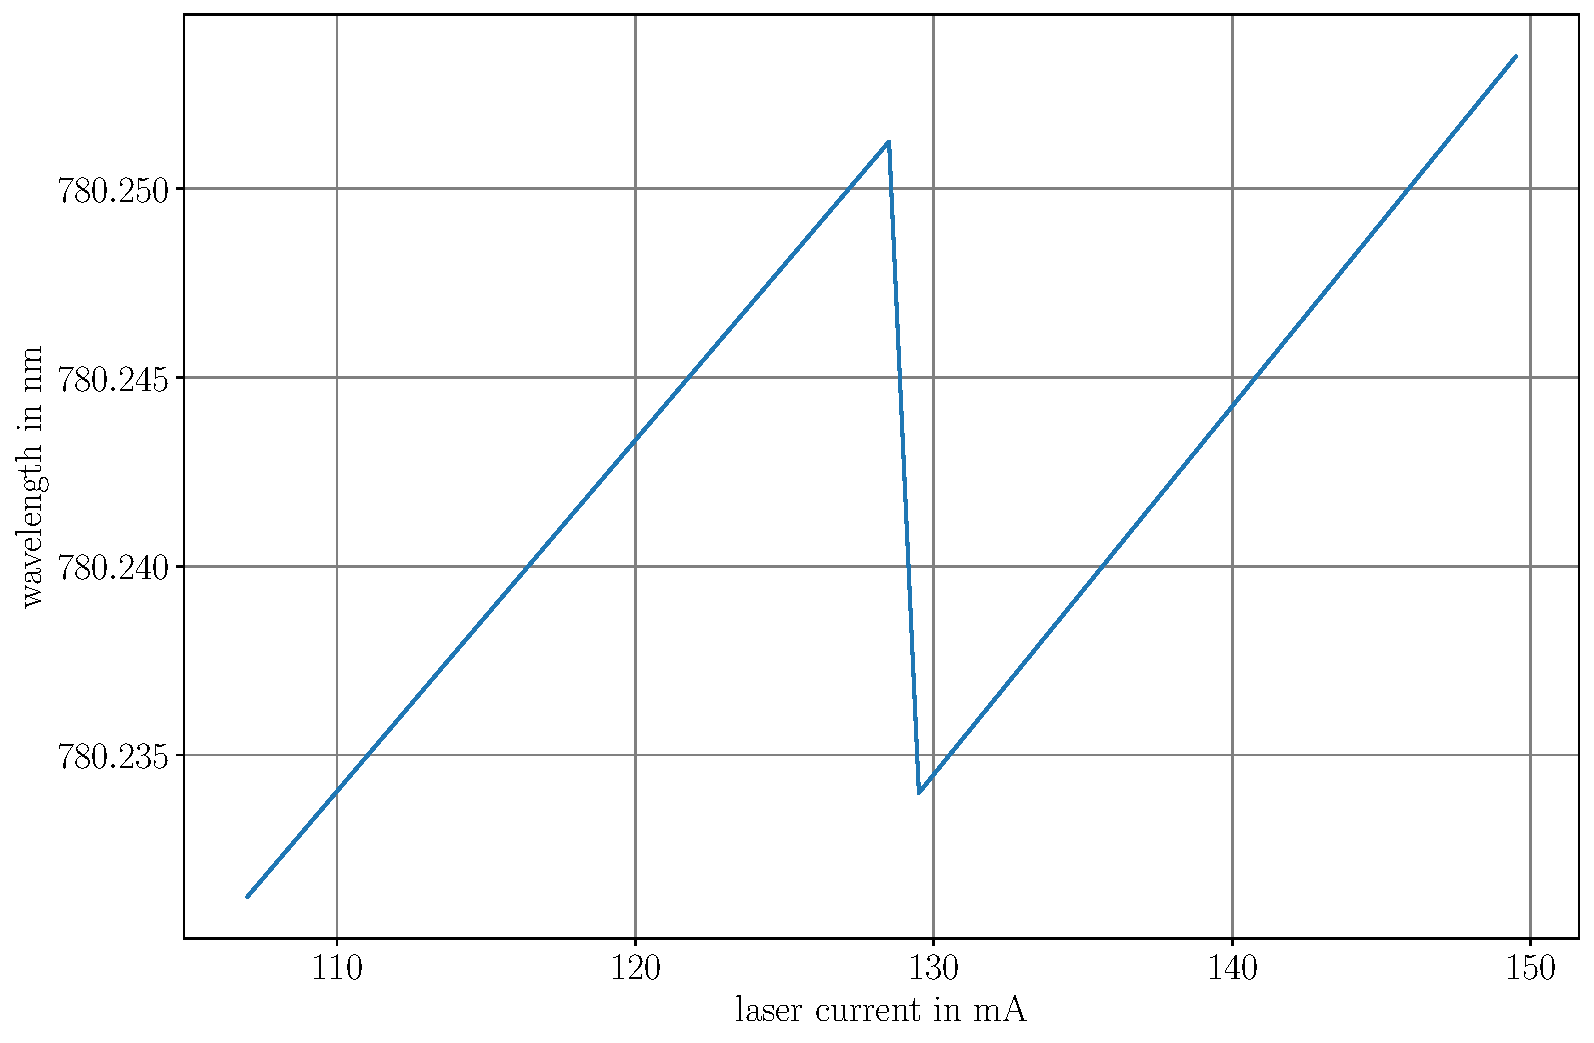
\includegraphics[scale=0.45]{Aufg-1/currentTuning.pdf}
    \captionof{figure}{Cut current wavelength curve from 105 mA to 150 mA using python}
    \label{image:currentTuningCut}
\end{center}
From the csv-file we can easily find our value for the peaks of the reference beam and convert them into the corresponding wavelength. Then we compared the measured wavelength with the literature there $F$ are the quantum number of the $5^2S_{1/2}$-state.
\begin{center}
    \begin{tabular}{c | c | c c c | c c }
        \makecell{Peak\\order} & \makecell{laser\\current/mA} & \makecell{wavelength\\measured/nm} & \makecell{wavelength\\literature/nm} & deviation/nm & isotope & $F$ \\
        \hline
        1 & 119.4429 & 780.243 & 780.233 & 0.010 & $^{87}Rb$ & 1 \\
        2 & 125.0267 & 780.248 & 780.238 & 0.010 & $^{85}Rb$ & 2 \\
        3 & 131.8581 & 780.236 & 780.244 & 0.008 & $^{85}Rb$ & 3 \\
        4 & 134.7829 & 780.239 & 780.246 & 0.007 & $^{87}Rb$ & 2 \\       
    \end{tabular}
    \captionof{table}{Identification by intensity and order}
    \label{tab:identify}
\end{center}
Because $^{85}Rb$ have to be isotope with the highest occurrence we can clearly identify the highest peaks of the absorption spectrum as the one of $^{85}Rb$. In addition to that we can conclude that the measured data have some kind of bias, roughly 0.010 nm, in each area of the current wavelength curve of the laser.